\subsection{Pipeline View}
\label{sec:pipeline}
The pipeline view provides a direct visual representation of the three stages (encoder, attention, classifier) of the model. In the proposed tool, we allow model parameters to be updated (via an optimization) to correct a prediction error (\textbf{T3}). The pipeline view, by visualizing the distribution of the parameter changes, informs the user about how each stage responds to the optimization.

There are many ways to update the model to correct a prediction. The simplest approach is applying standard backpropagation and overfits to the example. However, without any constraint, the update step may alter the model in unexpected ways.
% \shusen{what is the benefit of using mira?}
Instead, we adopt the idea in the \emph{margin-infused relaxed algorithm (MIRA)}~\cite{CrammerSinger2003}, where we regulate the optimization with the L2-norm of the parameter change. In the proposed tool, we obtain the target parameters by the following optimization:
\vspace{-0.3mm}
\begin{equation}
\vspace{-1.2mm}
\underset{\mathbf{W}'}{\mathrm{argmin}}( C \mathbb{J}(\mathbf{W}') + ||\mathbf{W}' - \mathbf{W_o}||^2)
%\vspace{-0.5mm}
\end{equation}

where $\mathbb{J}(\mathbf{W})$ is the loss function of the neural network model, $\mathbf{W_o}$ is the original model's parameters taken as constant, $\mathbf{W}'$ is the updated parameters, and $C$ is the weighting term, which determines whether we intended to emphasize more on obtaining better fitting or deviating less from the original model. Due to the nonconvex nature of the neural networks, we use SGD to optimize the above combined loss function.
%
With this formulation, we try to find a good approximation to the newly assigned label, while still maintaining relatively small changes with respect to the original model.

\begin{figure}[htbp]
\centering
\vspace{-3mm}
 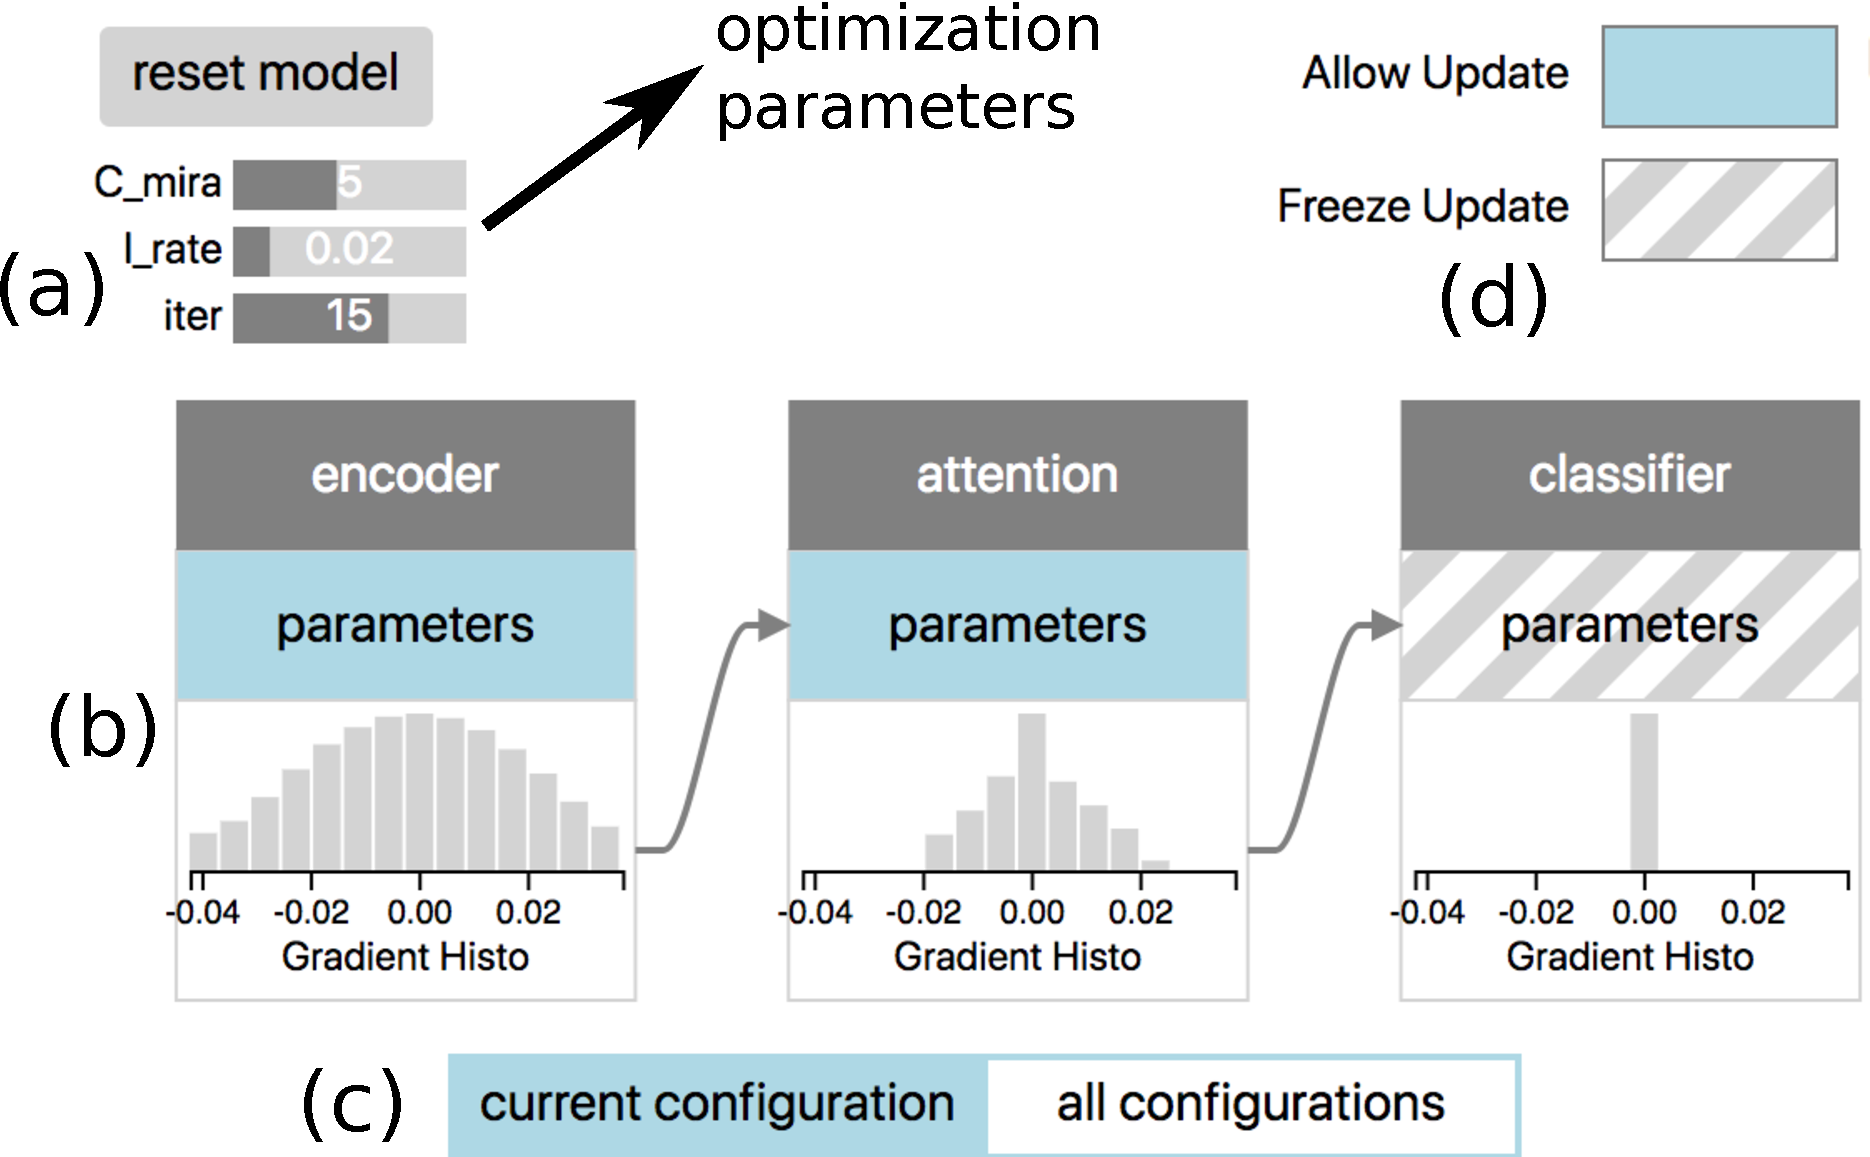
\includegraphics[width=0.9\linewidth]{pipelineView}
 \vspace{-2mm}
 \caption{
The pipeline view provides the visual representation of the three stages (encoder, attention, classifier) of the NLI model. 
%
In the proposed tool, we allow model parameters to be updated to correct a prediction error via a constrained optimization.
The hyperparameters for this optimization are shown in (a). 
In (b), we utilize a graphical representation for each stage of the pipeline.
% where the user can click on the blue rectangle marked with the word ``parameter'' to enable or disable its update (the legend is shown in (d)). 
In (c), the user can select whether to use the current pipeline configuration as displayed or try all the pipeline configuration combinations for the optimization. %whether we want to use the current pipeline configuration as displayed or try all the pipeline configuration combinations as the parameter update operation can be enabled or disabled for each stage.
}
\label{fig:pipelineView}
\vspace{-2mm}
\end{figure}

The optimization hyperparameters are shown in Fig.~\ref{fig:pipelineView}(a). Each stage is illustrated by a glyph (Fig.~\ref{fig:pipelineView}(b)), in which the user can enable or disable its parameter update by clicking on the blue rectangle marked with the word ``parameter'' (the legend about its state is shown in Fig.~\ref{fig:pipelineView}(d)). In Fig.~\ref{fig:pipelineView}(c), we select whether we want to use the current pipeline update setting as displayed or try all the pipeline configuration combinations (i.e., each stage can be either enabled or disabled; therefore, there are $8$ combinations in total, or $7$ if we discard the case where all stages are not enabled).



% \textbf{Margin-Infused Relaxed Algorithm (MIRA)}
